\documentclass[a4paper]{article}

\usepackage[spanish]{babel} % Le indicamos a LaTeX que vamos a escribir en espa�ol.
\usepackage[latin1]{inputenc} % Permite utilizar tildes y e�es normalmente
\usepackage{pdfpages}
%\usepackage{framed}
\usepackage{ifthen}
\usepackage{amssymb}
\usepackage{multicol}
\usepackage{graphicx}
\usepackage[absolute]{textpos}
\makeatletter

\@ifclassloaded{beamer}{%
  \newcommand{\tocarEspacios}{%
    \addtolength{\leftskip}{4em}%
    \addtolength{\parindent}{-3em}%
  }%
}
{%
  \usepackage[top=1cm,bottom=2cm,left=1cm,right=1cm]{geometry}%
  \usepackage{color}%
  \newcommand{\tocarEspacios}{%
    \addtolength{\leftskip}{5em}%
    \addtolength{\parindent}{-3em}%
  }%
}

\newcommand{\encabezadoDeProblema}[4]{%
  % Ponemos la palabrita problema en tt
%  \noindent%
  {\normalfont\bfseries\ttfamily problema}%
  % Ponemos el nombre del problema
  \ %
  {\normalfont\ttfamily #2}%
  \ 
  % Ponemos los parametros
  (#3)%
  \ifthenelse{\equal{#4}{}}{}{%
  \ =\ %
  % Ponemos el nombre del resultado
  {\normalfont\ttfamily #1}%
  % Por ultimo, va el tipo del resultado
  \ : #4}
}

\newcommand{\encabezadoDeTipo}[2]{%
  % Ponemos la palabrita tipo en tt
  {\normalfont\bfseries\ttfamily tipo}%
  % Ponemos el nombre del tipo
  \ %
  {\normalfont\ttfamily #2}%
  \ifthenelse{\equal{#1}{}}{}{$\langle$#1$\rangle$}
}

% Primero definiciones de cosas al estilo title, author, date

\def\materia#1{\gdef\@materia{#1}}
\def\@materia{No especifi\'o la materia}
\def\lamateria{\@materia}

\def\cuatrimestre#1{\gdef\@cuatrimestre{#1}}
\def\@cuatrimestre{No especifi\'o el cuatrimestre}
\def\elcuatrimestre{\@cuatrimestre}

\def\anio#1{\gdef\@anio{#1}}
\def\@anio{No especifi\'o el anio}
\def\elanio{\@anio}

\def\fecha#1{\gdef\@fecha{#1}}
\def\@fecha{\today}
\def\lafecha{\@fecha}

\def\nombre#1{\gdef\@nombre{#1}}
\def\@nombre{No especific'o el nombre}
\def\elnombre{\@nombre}

\def\practicas#1{\gdef\@practica{#1}}
\def\@practica{No especifi\'o el n\'umero de pr\'actica}
\def\lapractica{\@practica}


% Esta macro convierte el numero de cuatrimestre a palabras
\newcommand{\cuatrimestreLindo}{
  \ifthenelse{\equal{\elcuatrimestre}{1}}
  {Primer cuatrimestre}
  {\ifthenelse{\equal{\elcuatrimestre}{2}}
  {Segundo cuatrimestre}
  {Verano}}
}


\newcommand{\depto}{{UBA -- Facultad de Ciencias Exactas y Naturales --
      Departamento de Computaci\'on}}

\newcommand{\titulopractica}{
  \centerline{\depto}
  \vspace{1ex}
  \centerline{{\Large\lamateria}}
  \vspace{0.5ex}
  \centerline{\cuatrimestreLindo de \elanio}
  \vspace{2ex}
  \centerline{{\huge Pr\'actica \lapractica -- \elnombre}}
  \vspace{5ex}
  \arreglarincisos
  \newcounter{ejercicio}
  \newenvironment{ejercicio}{\stepcounter{ejercicio}\textbf{Ejercicio
      \theejercicio}%
    \renewcommand\@currentlabel{\theejercicio}%
  }{\vspace{0.2cm}}
}  


\newcommand{\titulotp}{
  \centerline{\depto}
  \vspace{1ex}
  \centerline{{\Large\lamateria}}
  \vspace{0.5ex}
  \centerline{\cuatrimestreLindo de \elanio}
  \vspace{0.5ex}
  \centerline{\lafecha}
  \vspace{2ex}
  \centerline{{\huge\elnombre}}
  \vspace{5ex}
}


%practicas
\newcommand{\practica}[2]{%
    \title{Pr\'actica #1 \\ #2}
    \author{Algoritmos y Estructuras de Datos I}
    \date{Segundo Cuatrimestre 2015}

    \maketitlepractica{#1}{#2}
}

\newcommand \maketitlepractica[2] {%
\begin{center}
\begin{tabular}{r cr}
 \begin{tabular}{c}
{\large\bf\textsf{\ Algoritmos y Estructuras de Datos I\ }}\\ 
Segundo Cuatrimestre 2015\\
\title{\normalsize Gu\'ia Pr\'actica #1 \\ \textbf{#2}}\\
\@title
\end{tabular} &
\begin{tabular}{@{} p{1.6cm} @{}}
\includegraphics[width=1.6cm]{logodpt.jpg}
\end{tabular} &
\begin{tabular}{l @{}}
 \emph{Departamento de Computaci\'on} \\
 \emph{Facultad de Ciencias Exactas y Naturales} \\
 \emph{Universidad de Buenos Aires} \\
\end{tabular} 
\end{tabular}
\end{center}

\bigskip
}


% Simbolos varios

\newcommand{\ent}{\ensuremath{\mathbb{Z}}}
\newcommand{\float}{\ensuremath{\mathbb{R}}}
\newcommand{\bool}{\ensuremath{\mathsf{Bool}}}
\newcommand{\True}{\ensuremath{\mathrm{True}}}
\newcommand{\False}{\ensuremath{\mathrm{False}}}
\newcommand{\Then}{\ensuremath{\rightarrow}}
\newcommand{\Iff}{\ensuremath{\leftrightarrow}}
\newcommand{\implica}{\ensuremath{\longrightarrow}}
\newcommand{\IfThenElse}[3]{\ensuremath{\mathsf{if}\ #1\ \mathsf{then}\ #2\ \mathsf{else}\ #3}}


\newcommand{\rango}[2]{[#1\twodots#2]}
\newcommand{\comp}[2]{[\,#1\,|\,#2\,]}

\newcommand{\rangoac}[2]{(#1\twodots#2]}
\newcommand{\rangoca}[2]{[#1\twodots#2)}
\newcommand{\rangoaa}[2]{(#1\twodots#2)}

%ejercicios
\newtheorem{exercise}{Ejercicio}
\newenvironment{ejercicio}{\begin{exercise}\rm}{\end{exercise} \vspace{0.2cm}}
\newenvironment{items}{\begin{enumerate}[i)]}{\end{enumerate}}
\newenvironment{subitems}{\begin{enumerate}[a)]}{\end{enumerate}}
\newcommand{\sugerencia}[1]{\noindent \textbf{Sugerencia:} #1}

%tipos basicos
\newcommand{\rea}{\ensuremath{\mathsf{Float}}}
\newcommand{\cha}{\ensuremath{\mathsf{Char}}}

\newcommand{\mcd}{\mathrm{mcd}}
\newcommand{\prm}[1]{\ensuremath{\mathsf{prm}(#1)}}
\newcommand{\sgd}[1]{\ensuremath{\mathsf{sgd}(#1)}}

%listas
\newcommand{\TLista}[1]{[#1]}
\newcommand{\lvacia}{\ensuremath{[\ ]}}
\newcommand{\lv}{\ensuremath{[\ ]}}
\newcommand{\longitud}[1]{\left| #1 \right|}
\newcommand{\cons}[1]{\ensuremath{\mathsf{cons}}(#1)}
\newcommand{\indice}[1]{\ensuremath{\mathsf{indice}}(#1)}
\newcommand{\conc}[1]{\ensuremath{\mathsf{conc}}(#1)}
\newcommand{\cab}[1]{\ensuremath{\mathsf{cab}}(#1)}
\newcommand{\cola}[1]{\ensuremath{\mathsf{cola}}(#1)}
\newcommand{\sub}[1]{\ensuremath{\mathsf{sub}}(#1)}
\newcommand{\en}[1]{\ensuremath{\mathsf{en}}(#1)}
\newcommand{\cuenta}[2]{\mathsf{cuenta}\ensuremath{(#1, #2)}}
\newcommand{\suma}[1]{\mathsf{suma}(#1)}
\newcommand{\twodots}{\ensuremath{\mathrm{..}}}
\newcommand{\masmas}{\ensuremath{++}}

% Acumulador
\newcommand{\acum}[1]{\ensuremath{\mathsf{acum}}(#1)}
\newcommand{\acumselec}[3]{\ensuremath{\mathrm{acum}(#1 |  #2, #3)}}

% \selector{variable}{dominio}
\newcommand{\selector}[2]{#1~\ensuremath{\leftarrow}~#2}
\newcommand{\selec}{\ensuremath{\leftarrow}}


\newenvironment{problema}[4][res]{%
  % El parametro 1 (opcional) es el nombre del resultado
  % El parametro 2 es el nombre del problema
  % El parametro 3 son los parametros
  % El parametro 4 es el tipo del resultado
  % Preambulo del ambiente problema
  % Tenemos que definir los comandos requiere, asegura, modifica y aux
  \newcommand{\requiere}[2][]{%
    {\normalfont\bfseries\ttfamily requiere}%
    \ifthenelse{\equal{##1}{}}{}{\ {\normalfont\ttfamily ##1} :}\ %
    \ensuremath{##2}%
    {\normalfont\bfseries\,;\par}%
  }
  \newcommand{\asegura}[2][]{%
    {\normalfont\bfseries\ttfamily asegura}%
    \ifthenelse{\equal{##1}{}}{}{\ {\normalfont\ttfamily ##1} :}\
    \ensuremath{##2}%
    {\normalfont\bfseries\,;\par}%
  }
  \newcommand{\modifica}[1]{%
    {\normalfont\bfseries\ttfamily modifica\ }%
    \ensuremath{##1}%
    {\normalfont\bfseries\,;\par}%
  }
  \renewcommand{\aux}[4]{%
    {\normalfont\bfseries\ttfamily aux\ }%
    {\normalfont\ttfamily ##1}%
    \ifthenelse{\equal{##2}{}}{}{\ (##2)}\ : ##3\, = \ensuremath{##4}%
    {\normalfont\bfseries\,;\par}%
  }
  \newcommand{\res}{#1}
  \vspace{1ex}
  \noindent
  \encabezadoDeProblema{#1}{#2}{#3}{#4}
  % Abrimos la llave
  \{\par%
  \tocarEspacios
}
% Ahora viene el cierre del ambiente problema
{
  % Cerramos la llave
  \noindent\}
  \vspace{1ex}
}


  \newcommand{\aux}[4]{%
    {\normalfont\bfseries\ttfamily aux\ }%
    {\normalfont\ttfamily #1}%
    \ifthenelse{\equal{#2}{}}{}{\ (#2)}\ : #3\, = \ensuremath{#4}%
    {\normalfont\bfseries\,;\par}%
  }


\newcommand{\pre}[1]{\textsf{pre}\ensuremath{(#1)}}

\newcommand{\problemanom}[1]{\textsf{#1}}
\newcommand{\problemail}[3]{\textsf{problema #1}\ensuremath{(#2) = #3}}
\newcommand{\problemailsinres}[2]{\textsf{problema #1}\ensuremath{(#2)}}
\newcommand{\requiereil}[2]{\textsf{requiere #1: }\ensuremath{#2}}
\newcommand{\asegurail}[2]{\textsf{asegura #1: }\ensuremath{#2}}
\newcommand{\modificail}[1]{\textsf{modifica }\ensuremath{#1}}
\newcommand{\auxil}[2]{\textsf{aux }\ensuremath{#1 = #2}}
\newcommand{\auxilc}[4]{\textsf{aux }\ensuremath{#1( #2 ): #3 = #4}}
\newcommand{\auxnom}[1]{\textsf{aux }\ensuremath{#1}}

\newcommand{\comentario}[1]{{/*\ #1\ */}}

\newcommand{\nom}[1]{\ensuremath{\mathsf{#1}}}

% -----------------
% Tipos compuestos
% -----------------

\newcommand{\Pred}[1]{\mathit{#1}}
\newcommand{\TSet}[1]{\textsf{Conjunto}\ensuremath{\langle #1 \rangle}}
\newcommand{\TSetFinito}[1]{\textsf{Conjunto}\ensuremath{\langle #1 \rangle}}
\newcommand{\TRac}{\tiponom{Racional}}
\newcommand{\TVec}{\tiponom{Vector}}
\newcommand{\Func}[1]{\mathrm{#1}}
\newcommand{\cardinal}[1]{\left| #1 \right|}


\newcommand{\sinonimo}[2]{%
  \noindent%
  {\normalfont\bfseries\ttfamily tipo\ }%
  #1\ =\ #2%
  {\normalfont\bfseries\,;\par}
}

\newcommand{\enum}[2]{%
  \noindent%
  {\normalfont\bfseries\ttfamily tipo\ }%
  #1\ =\ #2%
  {\normalfont\bfseries\,;\par}
}

%~ \newenvironment{tipo}[1]{%
    %~ \vspace{0.2cm}
    %~ \textsf{tipo #1}\ensuremath{\{}\\
    %~ \begin{tabular}[l]{p{0.02\textwidth} p{0.02\textwidth} p{0.82 \textwidth}}
%~ }{%
    %~ \end{tabular}
%~ 
    %~ \ensuremath{\}}
    %~ \vspace{0.15cm}
%~ }
%~ 

\newenvironment{tipo}[2][]{%
  % Preambulo del ambiente tipo
  % Tenemos que definir los comandos observador (con requiere) y aux
  \newcommand{\observador}[3]{%
    {\normalfont\bfseries\ttfamily observador\ }%
    {\normalfont\ttfamily ##1}%
    \ifthenelse{\equal{##2}{}}{}{\ (##2)}\ : ##3%
    {\normalfont\bfseries\,;\par}%
  }
  \newcommand{\requiere}[2][]{{%
    \addtolength{\leftskip}{3em}%
    \setlength{\parindent}{-2em}%
    {\normalfont\bfseries\ttfamily requiere}%
    \ifthenelse{\equal{##1}{}}{}{\ {\normalfont\ttfamily ##1} :}\ 
    \ensuremath{##2}%
    {\normalfont\bfseries\,;\par}}
  }
  \newcommand{\explicacion}[1]{{%
    \addtolength{\leftskip}{3em}%
    \setlength{\parindent}{-2em}%
    \par \hspace{2.3em} ##1 %
    {\par}
    }
  }
  \newcommand{\invariante}[2][]{%
    {\normalfont\bfseries\ttfamily invariante}%
    \ifthenelse{\equal{##1}{}}{}{\ {\normalfont\ttfamily ##1} :}\ 
    \ensuremath{##2}%
    {\normalfont\bfseries\,;\par}%
  }
  \renewcommand{\aux}[4]{%
    {\normalfont\bfseries\ttfamily aux\ }%
    {\normalfont\ttfamily ##1}%
    \ifthenelse{\equal{##2}{}}{}{\ (##2)}\ : ##3\, = \ensuremath{##4}%
    {\normalfont\bfseries\,;\par}%
  }
  \vspace{1ex}
  \noindent
  \encabezadoDeTipo{#1}{#2}
  % Abrimos la llave
  \{\par%
  \tocarEspacios
}
% Ahora viene el cierre del ambiente tipo
{
  % Cerramos la llave
  \noindent\}
  \vspace{1ex}
}


%~ \newcommand{\observador}[3]{%
    %~ & \multicolumn{2}{p{0.85\textwidth}}{\textsf{observador #1}\ensuremath{(#2):#3}}\\%
    %~ }
    
%~ \newcommand{\observador}[3]{%
    %~ {\normalfont\bfseries\ttfamily observador\ }%
    %~ {\normalfont\ttfamily ##1}%
    %~ \ifthenelse{\equal{##2}{}}{}{\ (##2)}\ : ##3%
    %~ {\normalfont\bfseries\,;\par}%
%~ }
    

%~ \newcommand{\observadorconreq}[3]{
    %~ & \multicolumn{2}{p{0.85\textwidth}}{\textsf{observador #1}\ensuremath{(#2):#3 \{}}\\
%~ }
%~ \newcommand{\observadorconreqfin}{
    %~ & \multicolumn{2}{p{0.85\textwidth}}{\ensuremath{\}}}\\
%~ }
%~ \newcommand{\obsrequiere}[2][]{& & \textsf{requiere #1: }\ensuremath{#2};\\}
%~ 
%~ \newcommand{\explicacion}[1]{&& #1 \\}
%~ \newcommand{\invariante}[2][]{%
    %~ & \multicolumn{2}{p{0.85\textwidth}}{\textsf{invariante #1: }\ensuremath{#2}}\\%
%~ }
%~ \newcommand{\auxinvariante}[2]{
    %~ & \multicolumn{2}{p{0.85\textwidth}}{\textsf{aux }\ensuremath{#1 = #2}};\\
%~ }
%~ \newcommand{\auxiliar}[4]{
    %~ & \multicolumn{2}{p{0.85\textwidth}}{\textsf{aux }\ensuremath{#1(#2): #3 = #4}};\\
%~ }

\newcommand{\tiponom}[1]{\ensuremath{\mathsf{#1}}\xspace}
\newcommand{\obsnom}[1]{\ensuremath{\mathsf{#1}}}

% -----------------
% Ecuaciones de terminacion en funcional
% -----------------

\newenvironment{ecuaciones}{%
    $$
    \begin{array}{l @{\ /\ (} l @{,\ } l @{)\ =\ } l}
}{%
    \end{array}
    $$
}




\newcommand{\ecuacion}[4]{#1 & #2 & #3 & #4\\}

\newcommand{\concat}{\nom{concat}}

% Listas por comprension. El primer parametro es la expresion y el
% segundo tiene los selectores y las condiciones.
%*\newcommand{\comp}[2]{[\,#1\,|\,#2\,]}























% En las practicas/parciales usamos numeros arabigos para los ejercicios.
% Aca cambiamos los enumerate comunes para que usen letras y numeros
% romanos
\newcommand{\arreglarincisos}{%
  \renewcommand{\theenumi}{\alph{enumi}}
  \renewcommand{\theenumii}{\roman{enumii}}
  \renewcommand{\labelenumi}{\theenumi)}
  \renewcommand{\labelenumii}{\theenumii)}
}





%%%%%%%%%%%%%%%%%%%%%%%%%%%%%% PARCIAL %%%%%%%%%%%%%%%%%%%%%%%%
\let\@xa\expandafter
\newcommand{\tituloparcial}{\centerline{\depto -- \lamateria}
  \centerline{\elnombre -- \lafecha}%
  \setlength{\TPHorizModule}{10mm} % Fija las unidades de textpos
  \setlength{\TPVertModule}{\TPHorizModule} % Fija las unidades de
                                % textpos
  \arreglarincisos
  \newcounter{total}% Este contador va a guardar cuantos incisos hay
                    % en el parcial. Si un ejercicio no tiene incisos,
                    % cuenta como un inciso.
  \newcounter{contgrilla} % Para hacer ciclos
  \newcounter{columnainicial} % Se van a usar para los cline cuando un
  \newcounter{columnafinal}   % ejercicio tenga incisos.
  \newcommand{\primerafila}{}
  \newcommand{\segundafila}{}
  \newcommand{\rayitas}{} % Esto va a guardar los \cline de los
                          % ejercicios con incisos, asi queda mas bonito
  \newcommand{\anchodegrilla}{20} % Es para textpos
  \newcommand{\izquierda}{7} % Estos dos le dicen a textpos donde colocar
  \newcommand{\abajo}{2}     % la grilla
  \newcommand{\anchodecasilla}{0.4cm}
  \setcounter{columnainicial}{1}
  \setcounter{total}{0}
  \newcounter{ejercicio}
  \setcounter{ejercicio}{0}
  \renewenvironment{ejercicio}[1]
  {%
    \stepcounter{ejercicio}\textbf{\noindent Ejercicio \theejercicio. [##1
      puntos]}% Formato
    \renewcommand\@currentlabel{\theejercicio}% Esto es para las
                                % referencias
    \newcommand{\invariante}[2]{%
      {\normalfont\bfseries\ttfamily invariante}%
      \ ####1\hspace{1em}####2%
    }%
    \renewcommand{\problema}[5][result]{
      \encabezadoDeProblema{####1}{####2}{####3}{####4}\hspace{1em}####5}%
  }% Aca se termina el principio del ejercicio
  {% Ahora viene el final
    % Esto suma la cantidad de incisos o 1 si no hubo ninguno
    \ifthenelse{\equal{\value{enumi}}{0}}
    {\addtocounter{total}{1}}
    {\addtocounter{total}{\value{enumi}}}
    \ifthenelse{\equal{\value{ejercicio}}{1}}{}
    {
      \g@addto@macro\primerafila{&} % Si no estoy en el primer ej.
      \g@addto@macro\segundafila{&}
    }
    \ifthenelse{\equal{\value{enumi}}{0}}
    {% No tiene incisos
      \g@addto@macro\primerafila{\multicolumn{1}{|c|}}
      \bgroup% avoid overwriting somebody else's value of \tmp@a
      \protected@edef\tmp@a{\theejercicio}% expand as far as we can
      \@xa\g@addto@macro\@xa\primerafila\@xa{\tmp@a}%
      \egroup% restore old value of \tmp@a, effect of \g@addto.. is
      
      \stepcounter{columnainicial}
    }
    {% Tiene incisos
      % Primero ponemos el encabezado
      \g@addto@macro\primerafila{\multicolumn}% Ahora el numero de items
      \bgroup% avoid overwriting somebody else's value of \tmp@a
      \protected@edef\tmp@a{\arabic{enumi}}% expand as far as we can
      \@xa\g@addto@macro\@xa\primerafila\@xa{\tmp@a}%
      \egroup% restore old value of \tmp@a, effect of \g@addto.. is
      % global 
      % Ahora el formato
      \g@addto@macro\primerafila{{|c|}}%
      % Ahora el numero de ejercicio
      \bgroup% avoid overwriting somebody else's value of \tmp@a
      \protected@edef\tmp@a{\theejercicio}% expand as far as we can
      \@xa\g@addto@macro\@xa\primerafila\@xa{\tmp@a}%
      \egroup% restore old value of \tmp@a, effect of \g@addto.. is
      % global 
      % Ahora armamos la segunda fila
      \g@addto@macro\segundafila{\multicolumn{1}{|c|}{a}}%
      \setcounter{contgrilla}{1}
      \whiledo{\value{contgrilla}<\value{enumi}}
      {%
        \stepcounter{contgrilla}
        \g@addto@macro\segundafila{&\multicolumn{1}{|c|}}
        \bgroup% avoid overwriting somebody else's value of \tmp@a
        \protected@edef\tmp@a{\alph{contgrilla}}% expand as far as we can
        \@xa\g@addto@macro\@xa\segundafila\@xa{\tmp@a}%
        \egroup% restore old value of \tmp@a, effect of \g@addto.. is
        % global 
      }
      % Ahora armo las rayitas
      \setcounter{columnafinal}{\value{columnainicial}}
      \addtocounter{columnafinal}{-1}
      \addtocounter{columnafinal}{\value{enumi}}
      \bgroup% avoid overwriting somebody else's value of \tmp@a
      \protected@edef\tmp@a{\noexpand\cline{%
          \thecolumnainicial-\thecolumnafinal}}%
      \@xa\g@addto@macro\@xa\rayitas\@xa{\tmp@a}%
      \egroup% restore old value of \tmp@a, effect of \g@addto.. is
      \setcounter{columnainicial}{\value{columnafinal}}
      \stepcounter{columnainicial}
    }
    \setcounter{enumi}{0}%
    \vspace{0.2cm}%
  }%
  \newcommand{\tercerafila}{}
  \newcommand{\armartercerafila}{
    \setcounter{contgrilla}{1}
    \whiledo{\value{contgrilla}<\value{total}}
    {\stepcounter{contgrilla}\g@addto@macro\tercerafila{&}}
  }
  \newcommand{\grilla}{%
    \g@addto@macro\primerafila{&\textbf{TOTAL}}
    \g@addto@macro\segundafila{&}
    \g@addto@macro\tercerafila{&}
    \armartercerafila
    \ifthenelse{\equal{\value{total}}{\value{ejercicio}}}
    {% No hubo incisos
      \begin{textblock}{\anchodegrilla}(\izquierda,\abajo)
        \begin{tabular}{|*{\value{total}}{p{\anchodecasilla}|}c|}
          \hline
          \primerafila\\
          \hline
          \tercerafila\\
          \tercerafila\\
          \hline
        \end{tabular}
      \end{textblock}
    }
    {% Hubo incisos
      \begin{textblock}{\anchodegrilla}(\izquierda,\abajo)
        \begin{tabular}{|*{\value{total}}{p{\anchodecasilla}|}c|}
          \hline
          \primerafila\\
          \rayitas
          \segundafila\\
          \hline
          \tercerafila\\
          \tercerafila\\
          \hline
        \end{tabular}
      \end{textblock}
    }
  }%
  \vspace{0.4cm}
  \textbf{Nro. de orden:}
  
  \textbf{LU:}
  
  \textbf{Apellidos:}
  
  \textbf{Nombres:}
  \vspace{0.5cm}
}



% AMBIENTE CONSIGNAS
% Se usa en el TP para ir agregando las cosas que tienen que resolver
% los alumnos.
% Dentro del ambiente hay que usar \item para cada consigna

\newcounter{consigna}
\setcounter{consigna}{0}

\newenvironment{consignas}{%
  \newcommand{\consigna}{\stepcounter{consigna}\textbf{\theconsigna.}}%
  \renewcommand{\ejercicio}[1]{\item ##1 }
  \renewcommand{\problema}[5][result]{\item
    \encabezadoDeProblema{##1}{##2}{##3}{##4}\hspace{1em}##5}%
  \newcommand{\invariante}[2]{\item%
    {\normalfont\bfseries\ttfamily invariante}%
    \ ##1\hspace{1em}##2%
  }
  \renewcommand{\aux}[4]{\item%
    {\normalfont\bfseries\ttfamily aux\ }%
    {\normalfont\ttfamily ##1}%
    \ifthenelse{\equal{##2}{}}{}{\ (##2)}\ : ##3 \hspace{1em}##4%
  }
  % Comienza la lista de consignas
  \begin{list}{\consigna}{%
      \setlength{\itemsep}{0.5em}%
      \setlength{\parsep}{0cm}%
    }
}%
{\end{list}}



% para decidir si usar && o ^
\newcommand{\y}[0]{\ensuremath{\land}}

% macros de correctitud
\newcommand{\semanticComment}[2]{#1 \ensuremath{#2};}
\newcommand{\namedSemanticComment}[3]{#1 #2: \ensuremath{#3};}


\newcommand{\local}[1]{\semanticComment{local}{#1}}

\newcommand{\vale}[1]{\semanticComment{vale}{#1}}
\newcommand{\valeN}[2]{\namedSemanticComment{vale}{#1}{#2}}
\newcommand{\impl}[1]{\semanticComment{implica}{#1}}
\newcommand{\implN}[2]{\namedSemanticComment{implica}{#1}{#2}}
\newcommand{\estado}[1]{\semanticComment{estado}{#1}}

\newcommand{\invarianteCN}[2]{\namedSemanticComment{invariante}{#1}{#2}}
\newcommand{\invarianteC}[1]{\semanticComment{invariante}{#1}}
\newcommand{\varianteCN}[2]{\namedSemanticComment{variante}{#1}{#2}}
\newcommand{\varianteC}[1]{\semanticComment{variante}{#1}}
% Macros especificas para especificar problemas en AyEDI

\newcommand{\comen}[2]{%
\begin{framed}
\noindent \textsf{#1:} #2
\end{framed}
}
% Aca solo vamos a poner el esqueleto del documento, pero no vamos a especificar nada.

\begin{document} % Todo lo que escribamos a partir de aca va a aparecer en el documento.

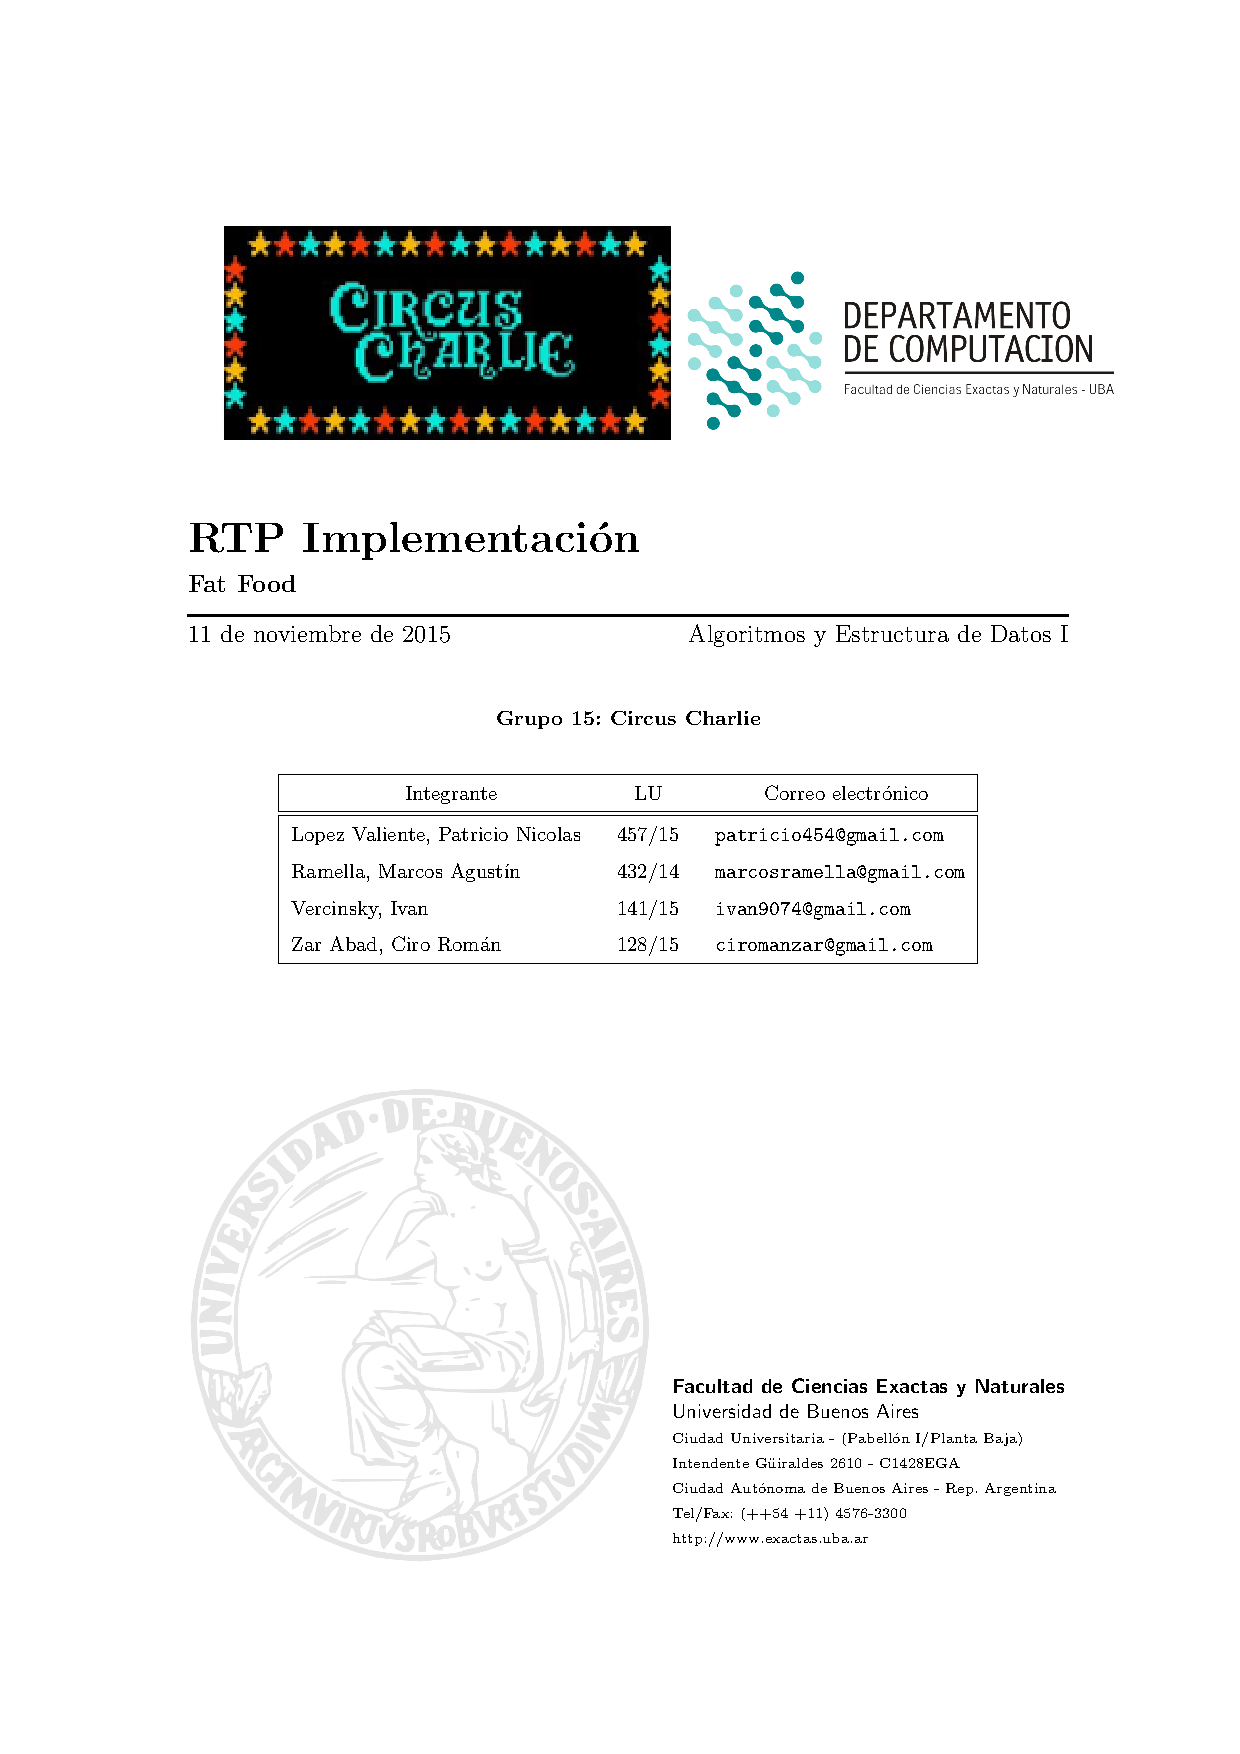
\includepdf{caratula}

\section{Tipos} %Defino los renombres de tipos b�sicos.

\sinonimo{Empleado}{String}
\sinonimo{Energia}{\ent}
\sinonimo{Cantidad}{\ent}
\enum{Bebida}{Pesti Cola, Falsa Naranja, Se ve nada, Agua con Gags, Agua sin Gags}
\enum{Hamburguesa}{McGyver, CukiQueFresco (Cuarto de Kilo con Queso Fresco), McPato, Big Macabra}


\section{Combo} %Defino el tipo combo, con su especificaci�n.

\begin{problema}{nuevoC}{b: Bebida, h: Hamburguesa, d: Energia}{Combo}
\requiere {energiaEnRango(d)}     
\asegura {bebida(res) == b}
\asegura {sandwich(res) == h}
\asegura {dificultad(res) == d}

\end{problema}

\begin{problema}{bebidaC}{c: Combo}{Bebida}
\asegura {res == Bebida(c)}
\end{problema}

\begin{problema}{sandwichC}{c: Combo}{Hamburguesa}
\asegura {res == sandwich(c)}
\end{problema}

\begin{problema}{dificultadC}{c: Combo}{Energia}
\asegura {res == dificultad(c)}
\end{problema} % Aca va la definici�n del tipo.

\begin{problema}{nuevoC}{b: Bebida, h: Hamburguesa, d: Energia}{Combo}
\requiere {energiaEnRango(d)}     
\asegura {bebida(res) == b}
\asegura {sandwich(res) == h}
\asegura {dificultad(res) == d}

\end{problema}

\begin{problema}{bebidaC}{c: Combo}{Bebida}
\asegura {res == Bebida(c)}
\end{problema}

\begin{problema}{sandwichC}{c: Combo}{Hamburguesa}
\asegura {res == sandwich(c)}
\end{problema}

\begin{problema}{dificultadC}{c: Combo}{Energia}
\asegura {res == dificultad(c)}
\end{problema} % La especificaci�n del tipo combo.

\newpage %Salto de p�gina


\section{Pedido} 

\begin{tipo}{Pedido}
	\observador{numero}{p: Pedido}{\ent}
	\observador{atendio}{p: Pedido}{Empleado}
	\observador{combos}{p: Pedido}{[Combo]}
	
	\medskip
	\invariante[numeroPositivo]{numero(p) > 0}
	\invariante[pideAlgo]{|combos(p)| > 0}
\end{tipo}




\begin{tipo}{Pedido}
	\observador{numero}{p: Pedido}{\ent}
	\observador{atendio}{p: Pedido}{Empleado}
	\observador{combos}{p: Pedido}{[Combo]}
	
	\medskip
	\invariante[numeroPositivo]{numero(p) > 0}
	\invariante[pideAlgo]{|combos(p)| > 0}
\end{tipo}




\newpage

\section{Local} 


\begin{problema}{stockBebidasL}{l: Local, b:Bebida}{Cantidad}
\requiere {b \in bebidasDelLocal(l)}
\asegura {stockBebidas(l, b) == res}
\end{problema}

\begin{problema}{stockSandwichesL}{l: Local, h:Hamburguesa}{Cantidad}
\requiere {h \in sandwichesDelLocal(l)}
\asegura {stockSandwiches(l, h) == res}
\end{problema}

\begin{problema}{bebidasDelLocalL}{l: Local}{[Bebida]}
\asegura {mismos(bebidasDelLocal(l), res)}
\end{problema}
	
\begin{problema}{sandwichesDelLocalL}{l: Local}{[Hamburguesa]}
\asegura {mismos(sandwichesDelLocal(l), res)}
\end{problema}

\begin{problema}{empleadosL}{l: Local}{[Empleado]}
\asegura {mismos(empleados(l), res)}
\end{problema}

\begin{problema}{desempleadosL}{l: Local}{[Empleado]}
\asegura {mismos(desempleados(l), res)}
\end{problema}

\begin{problema}{energiaEmpleadoL}{l: Local, e:Empleado}{Energia}
\requiere {e \in empleados(l)}
\asegura {energiaEmpleado(l, e) == res}
\end{problema}

\begin{problema}{ventasL}{l: Local}{[Pedido]}
\asegura {mismos(ventas(l), res)}
\end{problema}

\newpage

\begin{problema}{unaVentaCadaUno}{l:Local}{\bool}
\asegura [haySuficientesVentasYlasVentasRotan]{res == ((( \vert atendioEmpleado(l) \vert \geq \vert empleados(l) \vert) \wedge \\* ( \vert sacarRepeticiones(subventas(l)) \vert == \vert empleados(l) \vert )) \wedge \\* 
(\forall \ i \leftarrow [0.. \vert atendioEmpleado(l) \vert )) \ atendio(atendioEmpleado(l)_i) == atendio(subventas(l)[i \ mod \ \vert subventas(l) \vert ] ) \ ) }
\end{problema}

\begin{problema}{venderL}{l: Local, p:Pedido}{} 
\requiere [pedidoSeaCorrelativo]{(\vert ventas(p) \vert > 0) \Rightarrow numero(p) == NumeroPedidoUltimaVenta(l) + 1 }
\requiere [seaEmpleado]{atendio(p) \in empleados(l)}
\requiere [hayaStockDeBebidas]{\\ (\forall \ b \leftarrow bebidasDelPedido(p)) \ stockBebidas(l,b) \geq cuenta(b,bebidasDelPedido(p))}
\requiere [hayaStockDeSandwiches]{\\ (\forall \ s \leftarrow sandwichesDelPedido(p)) \ stockSandwiches(l,s) \geq cuenta(s,sandwichesDelPedido(p))}
\modifica {l}
\asegura [mantieneBebidas]{mismos(bebidasDelLocal(l),bebidasDelLocal(pre(l)))}
\asegura [mantieneSandwiches]{mismos(sandwichesDelLocal(l),sandwichesDelLocal(pre(l)))}	
\asegura [mantieneVentas]{mismos(ventas(l),p:ventas(pre(l)))}
\asegura [siTieneEnergiaParaVender]{energiaEmpleado(pre(l),atendio(p)) \geq dificultadPedido(p) \Rightarrow \\ mismos(empleados(pre(l)),empleados(l)) \wedge \\ 
	\ mismos(desempleados(pre(l)),desempleados(l)) \wedge \\
	\ energiaEmpleado(l,atendio(p)) ==  (energiaEmpleado(pre(l),atendio(p)) - dificultadPedido(p)) }
\asegura [siNoTieneEnergiaParaVender]{energiaEmpleado(pre(l),atendio(p)) < dificultadPedido(p) \Rightarrow \\ mismos(atendio(p):empleados(l),empleados(pre(l))  \wedge \\ mismos(desempleados(l),atendio(p):desempleados(pre(l)) ) }

\asegura [renuevaStockBebidas]{(\forall \ b \leftarrow bebidasDelLocal(pre(l))) \\ stockBebidas(l,b) == stockbebidas(pre(l),b) \ - \ cuenta(b,bebidasDelPedido(p))}
\asegura [renuevaStockSandwiches]{(\forall \ s \leftarrow sandwichesDelLocal(pre(l))) \\ stockSandwiches(l,s) == stockSandwiches(pre(l),s) \ - \ cuenta(s,sandwichesDelPedido)}
	
\end{problema}

\begin{problema}{candidatosAEmpleadosDelMesL}{l: Local}{[Empleado]}
\asegura [sonCandidatos]{mismos(res,[ \ e \ \vert \ e \selec empleadosConMasVentas(l), ( \forall \ e2 \selec empleadosConMasVentas(l)) \\  cantidadDeCombosDeEmpleado(e,l) \geq cantidadDeCombosDeEmpleado(e2,l) ] )}
\end{problema}


\begin{problema}{sancionL}{l: Local, e:Empleado, n:Energia}{}
\requiere [seaEmpleado]{e \in empleados(l)}
\requiere [energiaPositiva]{n > 0}
\modifica {l}
\asegura [mantieneVentas]{mismos(ventas(l),ventas(pre(l)))}
\asegura [mantieneBebidas]{mismos(bebidasDelLocal(l),bebidasDelLocal(pre(l)))}
\asegura [mantieneSandwiches]{mismos(sandwichesDelLocal(l),sandwichesDelLocal(pre(l)))}
\asegura [mantieneStockDeBebidas]{\\ (\forall \ b \leftarrow bebidasDelLocal(pre(l))) \  stockBebidas(l,b) == stockBebidas(pre(l),b)}
\asegura [mantieneStockDeSandwiches]{\\ (\forall \ s \leftarrow sandwichesDelLocal(pre(l))) \ stockSandwiches(l,s) == stockSandwiches(pre(l),s)}
\asegura [mantieneEnergiaDeOtrosEmpleados]{\\ (\forall \ x \leftarrow empleados(pre(l)), x \neq e) \ energiaEmpleado(l,x) == energiaEmpleado(pre(l),x)}
\asegura [siTieneEnergiaSuficiente]{energiaEmpleado(pre(l),e) \geq n \Rightarrow \\((mismos(empleados(l),empleados(pre(l))) \wedge \\ mismos(desempleados(l),desempleados(pre(l)))) \wedge \\ energiaEmpleado(l,e) == (energiaEmpleado(pre(l),e) - n))}
\asegura [sinoTieneEnergiaSuficiete]{energiaEmpleado(pre(l),e) < n \Rightarrow \\mismos(e:empleados(l),empleados(pre(l))) \wedge \\ mismos(desempleados(l),e:desempleados(pre(l)))}
\end{problema}



\begin{problema}{elVagonetaL}{l: Local}{Empleado}
\requiere [tengaVentas]{\vert ventas(l) \vert > 0}
\requiere [tengaEmpleados]{\vert empleados(l) \vert > 0}
\asegura [esUnVago]{res \in [ \ e \ \vert \ e \selec empleados(l) , (\forall \ e2 \selec empleados(l), e2 \neq e) \\* distanciaMayorEntreVentasDelEmpleado(e2, ventas(l)) \leq \\* distanciaMayorEntreVentasDelEmpleado(e, ventas(l)]}
\end{problema}

\newpage

\begin{problema}{anularPedidoL}{l: Local, n: \ent}{}
\requiere [esPedido]{n \in numVentaL(l)}
\requiere [atendioEmpleado]{atendio(ventaN(l,n)) \in empleados(l)}

\modifica {l}

\asegura [mantieneBebidas]{ mismos(bebidasDelLocal(l), bebidasDelLocal(pre(l)) ) }
\asegura [mantieneSandwiches]{ mismos(sandwichesDelLocal(l), sandwichesDelLocal(pre(l)) ) }
\asegura [mantieneEmpleados]{ mismos(empleados(l), empleados(pre(l)) ) } 
\asegura [mantieneDesempleados]{ mismos(desempleados(l), desempleados(pre(l)) ) } 

\asegura [mantieneLasOtrasVentas]{mismosVenta(ventas(l), ventaMenosN(pre(l),n))}

\asegura [mantieneCorrelatividad]{
mismos(sacarVentaN(pre(l),n),numVentaL(l))
}

\asegura [mantieneEnergiaOtrosEmpleados]{(\forall \ i \leftarrow empleados(l), i \neq atendio(ventaN(pre(l),n))) \\ energiaEmpleado(pre(l), i) == energiaEmpleado(l,i)
}

\asegura [actualizaEnergiaEmpleado]{\\
energiaEmpleado(pre(l), atendio(ventaN(pre(l),n))) \\ + \ dificultadPedido(ventaN(pre(l),n)) == energiaEmpleado(l, atendio(ventaN(pre(l),n)))
} 

\asegura [mantieneStockDeLasOtrasBebidas]{\\ (\forall \ i \leftarrow bebidasDelLocal(l), i \not\in bebidasUsadasN(pre(l),n) \\ stockBebidas(pre(l), i) == stockBebidas(l, i)} 


\asegura [actualizaStockBebidasDelPedidoAnulado]{\\
(\forall i \selec bebidasUsadasN(pre(l), n)) \\ stockBebidas(l, i) == stockBebidas(pre(l), i) + cuenta(i, bebidasN(pre(l), n))
}

\asegura [mantieneStockDeLosOtrosSandwiches]{\\ (\forall \ i \leftarrow sandwichesDelLocal(l), i \not\in sandwichesUsadosN(pre(l), n) \\ stockSandwiches(l, i) == stockSandwiches(pre(l), i)}


\asegura [actualizaStockSandwichesDelPedidoAnulado]{\\
(\forall i \selec sandwichesUsadosN(pre(l), n)) \\ stockSandwiches(l, i) == stockSandwiches(pre(l), i) + cuenta(i, sandwichesN(pre(l), n))
}


\end{problema}

\begin{problema}{agregarComboAlPedidoL}{l: Local, c: Combo, n:\ent}{}
\requiere [esPedido]{n \in numVentaL(l)}


\requiere [hayaBebidaDeC]{stockBebidas(l, bebida(c)) > 0}
\requiere [hayaSandwichDeC]{stockSandwiches(l, sandwich(c)) > 0}
\requiere [atendioEmpleado]{atendio(ventaN(l,n)) \in empleados(l)}
\requiere [tieneEnergiaParaC]{energiaEmpleado(l,atendio(ventaN(l,n)) \geq dificultad(c)}

\modifica {l}

\asegura [mantieneBebidas]{ mismos(bebidasDelLocal(l), bebidasDelLocal(pre(l)) ) }
\asegura [mantieneSandwiches]{ mismos(sandwichesDelLocal(l), sandwichesDelLocal(pre(l)) ) }
\asegura [mantieneEmpleados]{ mismos(empleados(l), empleados(pre(l)) ) } 
\asegura [mantieneDesempleados]{ mismos(desempleados(l), desempleados(pre(l)) ) } 

\asegura [lasOtrasVentasNoCambian]{\\
mismos(ventaMenosN(l,n), ventaMenosN(pre(l),n))
}
\asegura [mantieneNumeroVentaN]{
numero(ventaN(l,n)) == numero(ventaN(pre(l),n))
}
\asegura [mantieneEmpleadoVentaN]{
atendio(ventaN(l,n)) == atendio(ventaN(pre(l),n))
}
\asegura [agregaComboVentaN]{ 
combos(ventaN(l,n)) == combos(ventaN(pre(l),n)) ++ [c]
}

\asegura [mantieneStockDeLasOtrasBebidas]{\\ (\forall \ i \leftarrow bebidasDelLocal(l), i \neq bebida(c)) \ stockBebidas(pre(l), i) == stockBebidas(l, i) }

\asegura [actualizaStockBebidaC]{\\ 
stockBebidas(l, bebida(c)) == stockBebidas(pre(l), bebida(c)) - 1
}

\asegura [mantieneStockDeLosOtrosSandwiches]{\\
(\forall \ i \leftarrow sandwichesDelLocal(l), i \neq sandwich(c)) \ stockSandwiches(pre(l), i) == stockSandwiches(l, i) }

\asegura [actualizaStockSandwichC]{\\ 
stockSandwiches(l, sandwich(c)) == stockSandwiches(pre(l), sandwich(c)) - 1
}

\asegura [mantieneEnergiaDeLosOtrosEmpleados]{\\ (\forall \ i \leftarrow empleados(l), i \neq atendio(ventaN(l,n))) energiaEmpleado(pre(l), i) == energiaEmpleado(l,i)}

\asegura [actualizaEnergiaEmpleadoVentaN]{\\ energiaEmpleado(pre(l), atendio(ventaN(pre(l),n))) \ - \ dificultad (c) \\ == energiaEmpleado(l, atendio(ventaN(pre(l),n)))
}
\end{problema}


\begin{problema}{stockBebidasL}{l: Local, b:Bebida}{Cantidad}
\requiere {b \in bebidasDelLocal(l)}
\asegura {stockBebidas(l, b) == res}
\end{problema}

\begin{problema}{stockSandwichesL}{l: Local, h:Hamburguesa}{Cantidad}
\requiere {h \in sandwichesDelLocal(l)}
\asegura {stockSandwiches(l, h) == res}
\end{problema}

\begin{problema}{bebidasDelLocalL}{l: Local}{[Bebida]}
\asegura {mismos(bebidasDelLocal(l), res)}
\end{problema}
	
\begin{problema}{sandwichesDelLocalL}{l: Local}{[Hamburguesa]}
\asegura {mismos(sandwichesDelLocal(l), res)}
\end{problema}

\begin{problema}{empleadosL}{l: Local}{[Empleado]}
\asegura {mismos(empleados(l), res)}
\end{problema}

\begin{problema}{desempleadosL}{l: Local}{[Empleado]}
\asegura {mismos(desempleados(l), res)}
\end{problema}

\begin{problema}{energiaEmpleadoL}{l: Local, e:Empleado}{Energia}
\requiere {e \in empleados(l)}
\asegura {energiaEmpleado(l, e) == res}
\end{problema}

\begin{problema}{ventasL}{l: Local}{[Pedido]}
\asegura {mismos(ventas(l), res)}
\end{problema}

\newpage

\begin{problema}{unaVentaCadaUno}{l:Local}{\bool}
\asegura [haySuficientesVentasYlasVentasRotan]{res == ((( \vert atendioEmpleado(l) \vert \geq \vert empleados(l) \vert) \wedge \\* ( \vert sacarRepeticiones(subventas(l)) \vert == \vert empleados(l) \vert )) \wedge \\* 
(\forall \ i \leftarrow [0.. \vert atendioEmpleado(l) \vert )) \ atendio(atendioEmpleado(l)_i) == atendio(subventas(l)[i \ mod \ \vert subventas(l) \vert ] ) \ ) }
\end{problema}

\begin{problema}{venderL}{l: Local, p:Pedido}{} 
\requiere [pedidoSeaCorrelativo]{(\vert ventas(p) \vert > 0) \Rightarrow numero(p) == NumeroPedidoUltimaVenta(l) + 1 }
\requiere [seaEmpleado]{atendio(p) \in empleados(l)}
\requiere [hayaStockDeBebidas]{\\ (\forall \ b \leftarrow bebidasDelPedido(p)) \ stockBebidas(l,b) \geq cuenta(b,bebidasDelPedido(p))}
\requiere [hayaStockDeSandwiches]{\\ (\forall \ s \leftarrow sandwichesDelPedido(p)) \ stockSandwiches(l,s) \geq cuenta(s,sandwichesDelPedido(p))}
\modifica {l}
\asegura [mantieneBebidas]{mismos(bebidasDelLocal(l),bebidasDelLocal(pre(l)))}
\asegura [mantieneSandwiches]{mismos(sandwichesDelLocal(l),sandwichesDelLocal(pre(l)))}	
\asegura [mantieneVentas]{mismos(ventas(l),p:ventas(pre(l)))}
\asegura [siTieneEnergiaParaVender]{energiaEmpleado(pre(l),atendio(p)) \geq dificultadPedido(p) \Rightarrow \\ mismos(empleados(pre(l)),empleados(l)) \wedge \\ 
	\ mismos(desempleados(pre(l)),desempleados(l)) \wedge \\
	\ energiaEmpleado(l,atendio(p)) ==  (energiaEmpleado(pre(l),atendio(p)) - dificultadPedido(p)) }
\asegura [siNoTieneEnergiaParaVender]{energiaEmpleado(pre(l),atendio(p)) < dificultadPedido(p) \Rightarrow \\ mismos(atendio(p):empleados(l),empleados(pre(l))  \wedge \\ mismos(desempleados(l),atendio(p):desempleados(pre(l)) ) }

\asegura [renuevaStockBebidas]{(\forall \ b \leftarrow bebidasDelLocal(pre(l))) \\ stockBebidas(l,b) == stockbebidas(pre(l),b) \ - \ cuenta(b,bebidasDelPedido(p))}
\asegura [renuevaStockSandwiches]{(\forall \ s \leftarrow sandwichesDelLocal(pre(l))) \\ stockSandwiches(l,s) == stockSandwiches(pre(l),s) \ - \ cuenta(s,sandwichesDelPedido)}
	
\end{problema}

\begin{problema}{candidatosAEmpleadosDelMesL}{l: Local}{[Empleado]}
\asegura [sonCandidatos]{mismos(res,[ \ e \ \vert \ e \selec empleadosConMasVentas(l), ( \forall \ e2 \selec empleadosConMasVentas(l)) \\  cantidadDeCombosDeEmpleado(e,l) \geq cantidadDeCombosDeEmpleado(e2,l) ] )}
\end{problema}


\begin{problema}{sancionL}{l: Local, e:Empleado, n:Energia}{}
\requiere [seaEmpleado]{e \in empleados(l)}
\requiere [energiaPositiva]{n > 0}
\modifica {l}
\asegura [mantieneVentas]{mismos(ventas(l),ventas(pre(l)))}
\asegura [mantieneBebidas]{mismos(bebidasDelLocal(l),bebidasDelLocal(pre(l)))}
\asegura [mantieneSandwiches]{mismos(sandwichesDelLocal(l),sandwichesDelLocal(pre(l)))}
\asegura [mantieneStockDeBebidas]{\\ (\forall \ b \leftarrow bebidasDelLocal(pre(l))) \  stockBebidas(l,b) == stockBebidas(pre(l),b)}
\asegura [mantieneStockDeSandwiches]{\\ (\forall \ s \leftarrow sandwichesDelLocal(pre(l))) \ stockSandwiches(l,s) == stockSandwiches(pre(l),s)}
\asegura [mantieneEnergiaDeOtrosEmpleados]{\\ (\forall \ x \leftarrow empleados(pre(l)), x \neq e) \ energiaEmpleado(l,x) == energiaEmpleado(pre(l),x)}
\asegura [siTieneEnergiaSuficiente]{energiaEmpleado(pre(l),e) \geq n \Rightarrow \\((mismos(empleados(l),empleados(pre(l))) \wedge \\ mismos(desempleados(l),desempleados(pre(l)))) \wedge \\ energiaEmpleado(l,e) == (energiaEmpleado(pre(l),e) - n))}
\asegura [sinoTieneEnergiaSuficiete]{energiaEmpleado(pre(l),e) < n \Rightarrow \\mismos(e:empleados(l),empleados(pre(l))) \wedge \\ mismos(desempleados(l),e:desempleados(pre(l)))}
\end{problema}



\begin{problema}{elVagonetaL}{l: Local}{Empleado}
\requiere [tengaVentas]{\vert ventas(l) \vert > 0}
\requiere [tengaEmpleados]{\vert empleados(l) \vert > 0}
\asegura [esUnVago]{res \in [ \ e \ \vert \ e \selec empleados(l) , (\forall \ e2 \selec empleados(l), e2 \neq e) \\* distanciaMayorEntreVentasDelEmpleado(e2, ventas(l)) \leq \\* distanciaMayorEntreVentasDelEmpleado(e, ventas(l)]}
\end{problema}

\newpage

\begin{problema}{anularPedidoL}{l: Local, n: \ent}{}
\requiere [esPedido]{n \in numVentaL(l)}
\requiere [atendioEmpleado]{atendio(ventaN(l,n)) \in empleados(l)}

\modifica {l}

\asegura [mantieneBebidas]{ mismos(bebidasDelLocal(l), bebidasDelLocal(pre(l)) ) }
\asegura [mantieneSandwiches]{ mismos(sandwichesDelLocal(l), sandwichesDelLocal(pre(l)) ) }
\asegura [mantieneEmpleados]{ mismos(empleados(l), empleados(pre(l)) ) } 
\asegura [mantieneDesempleados]{ mismos(desempleados(l), desempleados(pre(l)) ) } 

\asegura [mantieneLasOtrasVentas]{mismosVenta(ventas(l), ventaMenosN(pre(l),n))}

\asegura [mantieneCorrelatividad]{
mismos(sacarVentaN(pre(l),n),numVentaL(l))
}

\asegura [mantieneEnergiaOtrosEmpleados]{(\forall \ i \leftarrow empleados(l), i \neq atendio(ventaN(pre(l),n))) \\ energiaEmpleado(pre(l), i) == energiaEmpleado(l,i)
}

\asegura [actualizaEnergiaEmpleado]{\\
energiaEmpleado(pre(l), atendio(ventaN(pre(l),n))) \\ + \ dificultadPedido(ventaN(pre(l),n)) == energiaEmpleado(l, atendio(ventaN(pre(l),n)))
} 

\asegura [mantieneStockDeLasOtrasBebidas]{\\ (\forall \ i \leftarrow bebidasDelLocal(l), i \not\in bebidasUsadasN(pre(l),n) \\ stockBebidas(pre(l), i) == stockBebidas(l, i)} 


\asegura [actualizaStockBebidasDelPedidoAnulado]{\\
(\forall i \selec bebidasUsadasN(pre(l), n)) \\ stockBebidas(l, i) == stockBebidas(pre(l), i) + cuenta(i, bebidasN(pre(l), n))
}

\asegura [mantieneStockDeLosOtrosSandwiches]{\\ (\forall \ i \leftarrow sandwichesDelLocal(l), i \not\in sandwichesUsadosN(pre(l), n) \\ stockSandwiches(l, i) == stockSandwiches(pre(l), i)}


\asegura [actualizaStockSandwichesDelPedidoAnulado]{\\
(\forall i \selec sandwichesUsadosN(pre(l), n)) \\ stockSandwiches(l, i) == stockSandwiches(pre(l), i) + cuenta(i, sandwichesN(pre(l), n))
}


\end{problema}

\begin{problema}{agregarComboAlPedidoL}{l: Local, c: Combo, n:\ent}{}
\requiere [esPedido]{n \in numVentaL(l)}


\requiere [hayaBebidaDeC]{stockBebidas(l, bebida(c)) > 0}
\requiere [hayaSandwichDeC]{stockSandwiches(l, sandwich(c)) > 0}
\requiere [atendioEmpleado]{atendio(ventaN(l,n)) \in empleados(l)}
\requiere [tieneEnergiaParaC]{energiaEmpleado(l,atendio(ventaN(l,n)) \geq dificultad(c)}

\modifica {l}

\asegura [mantieneBebidas]{ mismos(bebidasDelLocal(l), bebidasDelLocal(pre(l)) ) }
\asegura [mantieneSandwiches]{ mismos(sandwichesDelLocal(l), sandwichesDelLocal(pre(l)) ) }
\asegura [mantieneEmpleados]{ mismos(empleados(l), empleados(pre(l)) ) } 
\asegura [mantieneDesempleados]{ mismos(desempleados(l), desempleados(pre(l)) ) } 

\asegura [lasOtrasVentasNoCambian]{\\
mismos(ventaMenosN(l,n), ventaMenosN(pre(l),n))
}
\asegura [mantieneNumeroVentaN]{
numero(ventaN(l,n)) == numero(ventaN(pre(l),n))
}
\asegura [mantieneEmpleadoVentaN]{
atendio(ventaN(l,n)) == atendio(ventaN(pre(l),n))
}
\asegura [agregaComboVentaN]{ 
combos(ventaN(l,n)) == combos(ventaN(pre(l),n)) ++ [c]
}

\asegura [mantieneStockDeLasOtrasBebidas]{\\ (\forall \ i \leftarrow bebidasDelLocal(l), i \neq bebida(c)) \ stockBebidas(pre(l), i) == stockBebidas(l, i) }

\asegura [actualizaStockBebidaC]{\\ 
stockBebidas(l, bebida(c)) == stockBebidas(pre(l), bebida(c)) - 1
}

\asegura [mantieneStockDeLosOtrosSandwiches]{\\
(\forall \ i \leftarrow sandwichesDelLocal(l), i \neq sandwich(c)) \ stockSandwiches(pre(l), i) == stockSandwiches(l, i) }

\asegura [actualizaStockSandwichC]{\\ 
stockSandwiches(l, sandwich(c)) == stockSandwiches(pre(l), sandwich(c)) - 1
}

\asegura [mantieneEnergiaDeLosOtrosEmpleados]{\\ (\forall \ i \leftarrow empleados(l), i \neq atendio(ventaN(l,n))) energiaEmpleado(pre(l), i) == energiaEmpleado(l,i)}

\asegura [actualizaEnergiaEmpleadoVentaN]{\\ energiaEmpleado(pre(l), atendio(ventaN(pre(l),n))) \ - \ dificultad (c) \\ == energiaEmpleado(l, atendio(ventaN(pre(l),n)))
}
\end{problema}

\newpage

\section{Funciones Auxiliares}

\aux{distintos}{ls:[T]}{\bool}{ 
  (\forall \ i,j \selec [0..|ls|), i \neq j) \ ls_i \neq ls_j
}

\aux{energiaEnRango}{e: Energia} {\bool}{
        0 \leq e \leq 100
}

\aux{correlativos}{ls:[\ent]}{\bool}{
(((\forall \ n \leftarrow ls) (n+1) \in ls) \ \vee (esmax(n,ls))) \wedge (distintos(ls))
}

\aux{esmax}{n:\ent,ls:[\ent]}{\bool}{
(\forall \ x \leftarrow ls) \ n \geq x
}

\aux{sacarRepeticiones}{ls:[T]}{[T]}{
[ls_i \ \vert \ i \leftarrow [ 0.. \vert ls \vert) , ls_i \not \in ls(i..\vert ls \vert)] ] 
}

\aux{cuenta}{x:T, y:[T]}{\ent } {
\vert [i \ \vert \ i \selec y, i == x] \vert
}

\aux {maximo}{ls:[\ent]}{\ent}{
cab([x \ \vert \ x \leftarrow ls , (\forall \ y \leftarrow ls) \  x \geq y])
}

\subsection{Combo}
% los aux del tipo combo

\subsection{Pedido}
% los aux del tipo pedido
\aux{bebidasDelPedido}{p:Pedido}{[Bebida]}{
[bebida(combos(p)_i) \ \vert \ i \leftarrow [0..\vert combos(p) \vert) ]  
}
\aux{bebidasUsadas}{p:Pedido}{[Bebida]}{
sacarRepeticiones(bebidasDelPedido(p))  
}
\aux{sandwichesDelPedido}{p:Pedido}{[Hamburguesa]}{
[sandwich(combos(p)_i) \ \vert \ i \leftarrow [0..\vert combos(p) \vert) ]  
}
\aux{sandwichesUsados}{p:Pedido}{[Hamburguesa]}{
sacarRepeticiones(sandwichesDelPedido(p))  
}
\aux{dificultadPedido}{p:Pedido}{ \ent }{
\vert [ 1 \ \vert \ c \selec combos(p), i \selec [0.. dificultad(c)) ] \vert
}
\aux{cantidadMovimientos}{cs:[Combo], cs2:[Combo]}{\ent}{
\vert [1 \ \vert \ i \leftarrow [0..\vert cs \vert ), \neg combosIguales(cs_i ,cs2_i)] \vert 
}
\aux {combosIguales}{c1:Combo, c2:Combo}{\bool}{
(bebida(c1) == bebida(c2)) \wedge (sandwich(c1) == sandwich(c2))
}
\aux {vuelveAAparecer}{i: \ent , cs:[Combo]}{\bool}{
\vert [cs_x \ \vert \ x \selec (i.. \vert cs \vert ), combosIguales(cs_i,cs_x)] \vert > 0
}
\aux{cantRepeticionesDeCombos}{cs:[Combo]}{\ent}{
\vert [cs_i \ \vert \ i \selec [0.. \vert cs \vert ), vuelveAAparecer(i, cs)] \vert
}
\aux{distintosSyB}{cs:[Combo]}{\bool}{
(\forall \ i,j \selec [0..|cs|), i \neq j) \ \neg combosIguales(cs_i, cs_j)
}

\subsection{Local}
% los aux del tipo local
\aux{atendioEmpleado}{l:Local}{[Empleado]}{
[atendio(p) \ \vert \ p \leftarrow ventas(l), atendio(p) \in empleado(l)]
}
\aux{subventas}{l:Local}{[Empleado]}{
atendioEmpleado[0.. \vert empelados(l) \vert )
}

\aux{empleadosConMasVentas}{l:Local}{[Empleado]}{ 
[ \ e \  \vert \ e \leftarrow sacarRepeticiones(atendioEmpleado(l)),  \\ ( \forall \ e2 \leftarrow sacarRepeticiones(atendioEmpleado(l))) \ cuenta(e,atendioEmpleado(l)) \geq cuenta(e2,atendioEmpleado(l)) ]
}

\aux{cantidadDeCombosDeEmpleado}{e:Empleado, l:Local}{ \ent }{
 \\ \vert [ \ c \ \vert \ p \leftarrow ventas(l), \ c \leftarrow combos(p), \ atendio(p) == e] \vert
}

\aux{numVentaL}{l:Local}{[\ent]}{ 
[ \ numero(m) \  \vert \ m \leftarrow ventas(l)]
}

\aux{ventaN}{l:Local, n: \ent}{Pedido}{ 
cab([\ m \  \vert \ m \leftarrow ventas(l), numero(m) == n])
}

\aux{bebidasN}{l:Local, n:\ent}{[Bebida]}{
[bebida(i) \vert i \leftarrow combos(ventaN(l,n))]
}

\aux{bebidasUsadasN}{l:Local, n:\ent}{[Bebida]}{
sacarRepeticiones(bebidasN(l, n))
}

\aux{sandwichesN}{l:Local, n:\ent}{[Hamburguesa]}{
[sandwich(i) \vert i \leftarrow combos(ventaN(l,n)]
}

\aux{sandwichUsadosN}{l:Local, n:\ent}{[Hamburguesa]}{
sacarRepeticiones(sandwichesN(l, n))
}

\aux{ventasMenosN}{l:Local, n:\ent}{[Pedido]}{ 
[ p \vert p \leftarrow ventas(l), numero(p) \neq n]
}

\aux{mismosVenta}{l1:[Pedido], l2:[Pedido]}{\bool}{ 
|l1| == |l2| \wedge (\forall i \leftarrow l1) cuentaVenta(i, l1) == cuentaVenta(i, l2));
}

\aux{cuentaVenta}{x:Pedido, y:[Pedido]}{\ent } {
\vert [i \vert i \selec y, atendio(i) == atendio(x) \wedge combos(i) == combos(x)] \vert
}

\aux{ventasIguales}{v1:Pedido, v2:Pedido}{\bool}{
atendio(v1) == atendio(v2) \wedge \vert combos(v1) \vert == \vert combos(v2) \vert \wedge (\forall i \selec [0.. \vert combos(v1) \vert) \  combos(v1)_i == combos(v2)_i
}

\aux{NumeroPedidoUltimaVenta}{l:Local}{\ent}{
maximo([numero(p) \ \vert \ p \leftarrow ventas(l)])
}

\aux{posicionDeLaVenta}{e:Empleado, v:[Pedido]}{[\ent]}{
0:[(i+1) \ \vert \ i \selec [0..\vert v \vert), atendio(v_i) == e] ++ [\vert v \vert + 1]
}

\aux{distanciaEntreVentasDelEmpleado}{e:Empleado, v:[Pedido]}{[\ent]}{if \ \vert posicionDeLaVenta(e, v) \vert == 2 \ \\
then \ [\vert v \vert] \
else \ [(posicionDeLaVenta(e, v)_{i+1} - posicionDeLaVenta(e, v)_i -1) \vert i \selec [0..|posicionDeLaVenta(e, v)|-1)]}

\aux{distanciaMayorEntreVentasDelEmpleado}{e:Empleado, v:[Pedido]}{\ent}{ \\
maximo(distanciaEntreVentasDelEmpleado(e, v))
}


\aux{sacarVentaN}{l:Local,n:\ent}{[\ent]}{
[numero(i) \vert i \selec (numVentaL(l), numero(i) < n] ++ [numero(i)-1 \vert i \selec numVentaL(l), numero(i) > n]
}

\end{document} %Termin�!

